\documentclass[11pt]{article}
\usepackage{amsmath}
\usepackage{amssymb}
\usepackage{hyperref}
\usepackage{graphicx}
\usepackage{color}
\usepackage{cite}
\usepackage{framed}
\usepackage[margin=1in]{geometry}
\usepackage[parfill]{parskip}
\setlength{\parindent}{0pt}
\begin{document}

\title{Charge and Lattice Dynamics in Quantum Matter}
\author{Xunyang Hong}
\date{}
\maketitle





\begin{abstract}
This proposal presents a focused study on electron-phonon coupling in quantum matter using resonant inelastic X-ray scattering (RIXS) across three projects. \textbf{(1)} The first project aims to investigate the interaction between charge order and electron-phonon coupling in cuprate superconductors, particularly $\mathrm{La_{1.8-x}Eu_{0.2}Sr_xCuO_{4}}$, to understand interplay between phonons and charge order excitations. \textbf{(2)} The second project explores the electron-phonon dynamics in $\mathrm{SrTiO_{3}}$ and $\mathrm{KTaO_{3}}$, examining the reversed isotope effect and orientation-dependent superconductivity, respectively, by measurement of the electron-phonon coupling via RIXS. \textbf{(3)} Finally, the study extends to sapphire to measure its electron-phonon coupling, aiming to facilitate sub-MeV dark matter detection.

These projects collectively aim to deepen our understanding of electron-phonon interactions and their implications in superconductivity and dark matter research.
\end{abstract}

\section{Objectives of the project}
% \textit{\textbf{Instruction}: Please present the rationale for your project based on the current state of knowledge in the respective field, list the {\color{cyan}general research question} and the {\color{cyan}specific objectives}, mention the {\color{cyan}research methods}, and briefly discuss the {\color{cyan}expected results} and their implications for your field}

\paragraph{Research question and objectives}
Electron-phonon coupling is fundamental to the understanding of many phenomena in condensed matter physics, such as superconductivity\cite{bardeen_theory_1957,cuk_review_2005}, charge order\cite{arpaia_charge_2021,comin_resonant_2016,tranquada_spins_2013}, and even dark matter detection\cite{griffin_directional_2018}. 

In conventional superconductors that obey Bardeen-Cooper-Schrieffer (BCS) theory, phonon is believed to mediate the superconductivity\cite{bardeen_theory_1957}. Thus understanding electron-phonon coupling is crucial in conventional superconductivity. However, in high-temperature superconductors, despite the lack of a fully understood mechanism, studying the role of electron-phonon coupling in driving superconductivity remains intriguing.

In the course of my PhD. research, I propose 3 projects to study electron-phonon coupling in different systems, using the state-of-the-art high-resolution \textit{resonant inelastic x-ray scattering} (RIXS) technique\cite{ament_resonant_2011,zhou_i21_2022}. 

\paragraph{Project 1: Charge order and electron-phonon coupling in cuprate superconductors}
The coexistence and interaction of charge order with superconductivity phase remain not fully understood. The charge order phase is believed to compete against the superconductivity phase\cite{arpaia_charge_2021,comin_resonant_2016,canosa_resonant_2014, hucker_competing_2014, chang_direct_2012,ghiringhelli_long-range_2012}, but the underlying mechanism continues to be a mystery. A recent study suggested that the charge order in cuprate may also interact with phonons: (1) Electron-phonon coupling seems to reinforce the charge order in cuprate and result in a "lock-in" effect \cite{wang_charge_2021}; (2) phonon softening and intensity anomaly were observed near the charge order wavevector\cite{wang_charge_2021,lin_strongly_2020, huang_quantum_2021,miao_incommensurate_2018,tacon_inelastic_2014,li_multiorbital_2020,braicovich_determining_2020,chaix_dispersive_2017,peng_enhanced_2020};  However, Conversely, in a study I participated in, led by Prof. Johan Chang at University of Zurich, suggested the \textit{opposite}: phonons and charge order excitations are decoupled in $\mathrm{La_{2-x}Sr_xCuO_4}$.

This observed elusive relation among phonons, charge orders, and superconductivity underscores the significance of electron-phonon coupling. On one hand, electron-phonon coupling (especially its momentum dependence) determins how phonon can theoretically interact with charge order; on the other hand, both charge order and electron-phonon coupling play a role in shaping the behavior of superconductivity. Therefore, we propose exploring the electron-phonon coupling as well as how phonons interact with charge order in a $\mathrm{La_{1.8-x}Eu_{0.2}Sr_xCuO_{4}}$. We expect to unravel the mysterious relation between phonon and charge order in cuprate superconductors. 

\paragraph{Project 2: Electron-phonon coupling in $\mathrm{SrTiO_{3}}$ and $\mathrm{KTaO_{3}}$} 
$\mathrm{SrTiO_{3}}$ is a well-known superconducting material with a critical temperature of $\lesssim 1\, \mathrm{K}$\cite{schooley_superconductivity_1964,lin_fermi_2013}. Although it has a relatively simple crystal structure, the mechanism of superconductivity in $\mathrm{SrTiO_{3}}$ is still a mystery. Among all the puzzles, the most intriguing one is the reversed isotope effect: substitution of ${}^{16}\mathrm{O}$ by ${}^{18}\mathrm{O}$ surprisingly increases the critical temperature, contradicting the conventional BCS theory\cite{stucky_isotope_2016}. We propose investigating this effect by studying the electron-phonon coupling in $\mathrm{SrTiO_{3}}$ using RIXS. If the reversed isotope effect is also seen in electron-phonon coupling, it would be strong evidence that electron-phonon coupling plays a role in $\mathrm{SrTiO_{3}}$ superconductivity.

Another material of interest is $\mathrm{KTaO_{3}}$, which, though not superconducting in bulk, exhibits superconductivity on $\mathrm{LaAlO_{3}/KTaO_{3}}$ (LAO/KTO) interface, reported recently in Ref.\cite{ren_two-dimensional_2022}. However, unlike LAO/$\mathrm{SrTiO_{3}}$ interface where the superconductivity was found in all directions, the LAO/KTO interface exhibits a strong orientation-dependence of critical temperature\cite{ren_two-dimensional_2022,chen_two-dimensional_2021}. Similar to the hypothesis in $\mathrm{SrTiO_{3}}$, the orientation-dependent superconductivity observed in LAO/KTO might be attributed to the anisotropic electron-phonon coupling. To deepen our understanding, we aim to quantitatively and experimentally measure the electron-phonon coupling in LAO/KTO in different direction.


Therefore, we propose studying the isotope effect of electron-phonon coupling in $\mathrm{SrTiO_{3}}$, and the orientation dependence of electron-phonon coupling in LAO/KTO interface. Resonant inelastic X-ray scattering (RIXS) will be our main research tool. We expect to see a similar trend in electron-phonon coupling as in the superconducting critical temperature $T_{c}$, if electron-phonon coupling does play a role in superconductivity in these materials.



\paragraph{Project 3: Electron-phonon coupling in sapphire, a potential material for sub-MeV dark matter detection}
The concept of dark matter has long been shrouded in mystery in the field of modern physics. Despite numerous efforts to study and detect dark matter\cite{bergstrom_non-baryonic_2000,vogel_dark_2014,essig_first_2012,davidson_updated_2000}, the exact mass of the dark matter particle remains unknown. Various experimental tools have been utilized to cover a range of masses for dark matter detection. Phonon-based detector, for example, can be used to detect the sub-MeV dark matter (10 keV -- 1 MeV).
  
In dark matter models, dark matter particles interact with phonons, in a similar manner to electrons\cite{griffin_directional_2018}. Therefore, measuring the electron-phonon coupling is essential for advancing dark matter detection. Recent studies have identified sapphire as a suitable material for phonon-based dark matter detection, attributed to its polar nature, anisotropy, and minimal screening effect\cite{griffin_directional_2018}.
  
Therefore, we propose conducting a RIXS study on sapphire to experimentally extract the electron-phonon coupling. Accurate measurements of this coupling are expected to significantly facilitate the detection of dark matter using sapphire.

All of the above projects are based on the measurement of electron-phonon coupling. This requires the use of RIXS.
\begin{figure}[!t]
    \centering
    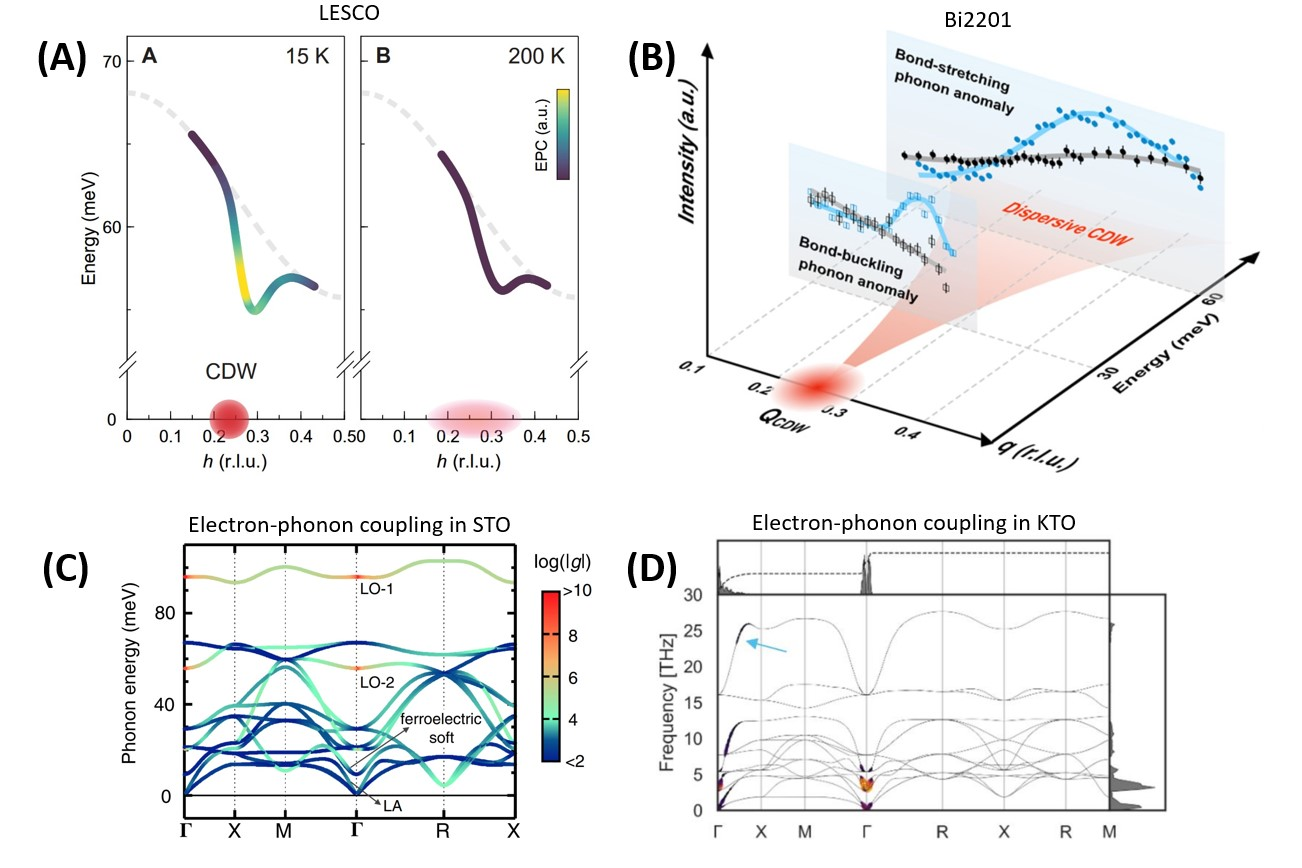
\includegraphics[width=0.9\textwidth]{figures/figure1.jpg}
    \caption{\textbf{(A)}: Dispersion of bond-stretching phonon in $\mathrm{La_{1.675}Eu_{0.2}Sr_{0.125}CuO_{4}}$. Phonon softening and Enhancement in electron-phonon coupling near charge order (CDW) observed in  through RIXS at Cu-L edge; The color in the curve indicates the extracted electron-phonon coupling (from Ref.\cite{wang_charge_2021}); \textbf{(B)} A sketch of phonon intensity as a function of momentum. Phonon intensity anomaly near charge order (CDW) observed in $\mathrm{Bi_2Sr_2LaCuO_{6+\delta}}$ through RIXS.  (from Ref.\cite{li_multiorbital_2020}); \textbf{(C)} and \textbf{(D)}: Theoretically calculated electron-phonon coupling in $\mathrm{SrTiO_3}$ and $\mathrm{KTaO_3}$ respectively. Strong coupling of longitudinal optical mode (LO) can be seen near $\Gamma$ point. Blue arrow points at the LO mode in  $\mathrm{KTaO_3}$ (from Ref.\cite{zhou_electron-phonon_2018} and Ref.\cite{esswein_first-principles_2023} respectively).}  
    \label{first_figure}
\end{figure}
\paragraph{Research method: resonant inelastic X-ray scattering (RIXS)}
The extraction of electron-phonon coupling has historically been challenging in condensed matter physics. Before the advent of RIXS, conventional experimental methods, such as neutron scattering or Raman scattering, are not directly related to the electron-phonon coupling. RIXS, on the other hand, enables a more direct extraction of the electron-phonon coupling. The concept of probing electron-phonon coupling using RIXS was first introduced by Ament et al. in 2011 \cite{ament_resonant_2011}. In their paper, they proposed a model to describe the phonon intensity in RIXS, with reasonable simplification and approximation. Later on, more sophisticated models were proposed to describe the phonon intensity in RIXS using Feynman diagrams \cite{devereaux_directly_2016,matsubayashi_numerical_2023} or density matrix renormalization group method\cite{nocera_computing_2018}, which allows us to \textit{simulate}  the RIXS spectrum, especially the spectrum with phonons. 

According to the theoretical models, phonon intensity in RIXS spectra is \textit{influenced} by the electron-phonon coupling\cite{devereaux_directly_2016}. In the case where electron-phonon coupling is independent of the momentum of the excited electron, the phonon intensity in the RIXS spectrum is \textit{directly proportional}  to the square of the electron-phonon coupling. Under the approximation that electron-phonon coupling is a constant, the \textit{relative} magnitude of the electron-phonon coupling can be calculated directly from the phonon intensity in the RIXS spectra. Additionally, the \textit{absolute} value of electron-phonon coupling can be further determined by either (1) comparing phonon intensity with its overtones; or (2) analyzing changes in phonon intensity upon detuning the incident energy\cite{ament_resonant_2011,braicovich_determining_2020}. Further development in RIXS theory proposes modification in Ament's model, accounting for the momentum dependence of electron-phonon coupling and relaxing some of its stringent assumptions in Ament's model\cite{bieniasz_theory_2022,geondzhian_generalization_2020}. 

It turns out that RIXS is a perfect tool for our projects due to its strong power in measuring phonons and electron-phonon coupling. Thanks to the recent development in RIXS, the resolution at copper-L edge and oxygen-K edge can reach up to $\sim 50\,\mathrm{meV}$ and $\sim 30\,\mathrm{meV}$ respectively, making it possible to separate phonon signal from pure elastic signal. Here we briefly summarize the use of RIXS in the three projects:
\begin{itemize}
  \item In project 1 (cuprate superconductor project), both charge order and phonons can be observed by RIXS. By simulating phonon and charge order spectrum separately, we can study the interplay between phonons and charge order. 
  \item In project 2 (STO and KTO project) and project 3 (sapphire project), the use of RIXS is more straightforward: acquiring the RIXS spectrum and directly extracting the electron-phonon coupling using Ament's model.
\end{itemize}


\begin{figure}[!t]
    \centering
    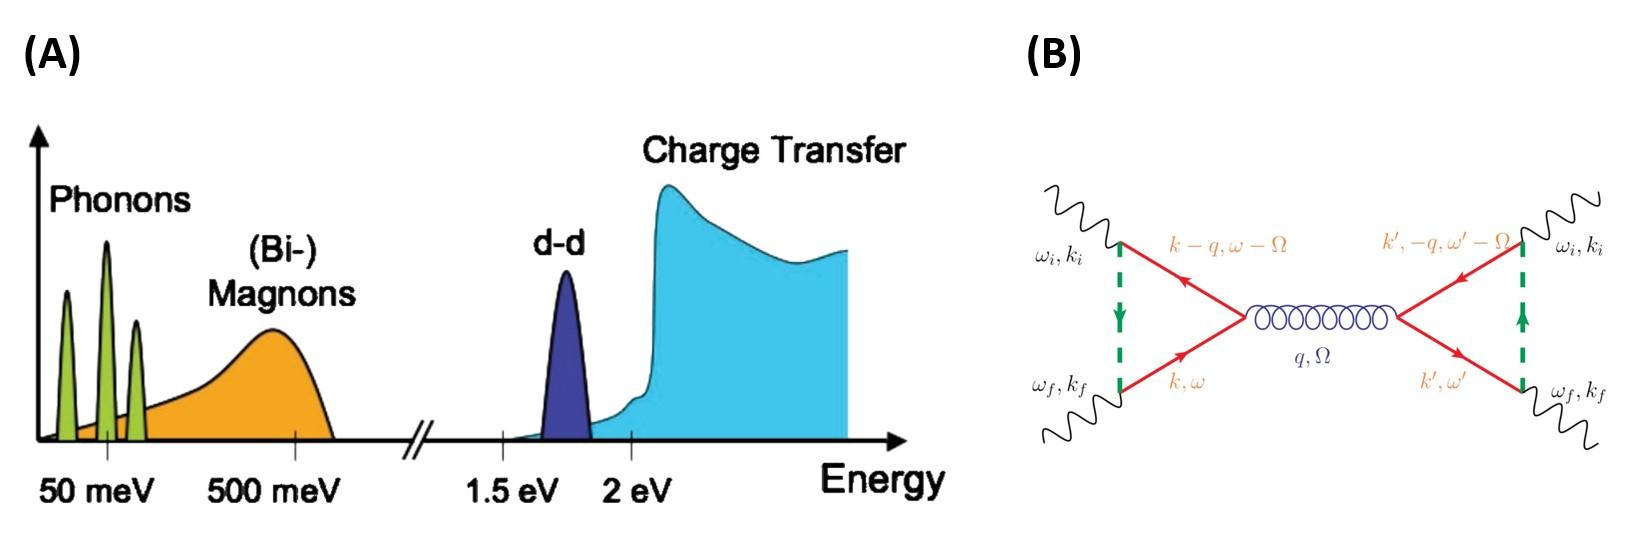
\includegraphics[width=0.9\textwidth]{figures/figure2.jpg}
    \caption{\textbf{(A)}: A sketch of possible excitations seen by RIXS. On the low-energy region there is phonons, which is our main focus in the projects (from Ref.\cite{ament_resonant_2011}); \textbf{B}: Feynman diagram of the RIXS process that generates phonons. Wavy lines represent photons, solid lines are electrons, and string-like line depicts phonon. It's clear from the diagram that electron-phonon coupling directly affects the cross section of the process (from Ref.\cite{devereaux_directly_2016}).}  
    \label{second_figure}
\end{figure}

\section{Background Information and Current State of Research}
% \textit{\textbf{Instructions}: Describe your project in the context of the {\color{cyan}current state of research} in your field. Refer to the most important publications, especially by other authors. {\color{cyan}Describe which previous findings are the starting point and basis for the planned studies}, where and why there is a need for research and which important, relevant research is currently underway in Switzerland and abroad. } 

The first superconductor was discovered in mercury (Hg) in 1911 by Kamerlingh Onnes. Since then, superconductivity has been observed in many materials, and the mechanism of superconductivity has been studied extensively. In 1957, Bardeen, Cooper, and Schrieffer introduced the BCS theory, the first successful theoretical framework to explain superconductivity\cite{bardeen_theory_1957}. In BCS theory, phonons are believed to mediate the superconductivity. More specifically, the interaction between phonons and electrons fosters an effective attractive force among electrons, leading to the formation of Cooper pairs, which are responsible for superconductivity at low temperatures\cite{bardeen_theory_1957}. 

In 1986, Bednorz and Müller discovered a lanthanum-based (La-based) cuprate material that became superconducting at a striking $35\,\mathrm{K}$\cite{bednorz_possible_1986}, heralding a new era of high-temperature superconductors. Since then, many  high-temperature superconductors have been discovered, including $\mathrm{YBa_{2}Cu_{3}O_{7-x}}$\cite{wu_superconductivity_1987}, $\mathrm{Bi_2Sr_2CaCu_{2}O_{8+x}}$\cite{maeda_a_1988}, and more. However, BCS theory falls short in explaining this type of superconductivity, with its underlying mechanism still being a subject of intense debate. Many new theories haven been put forward afterwards, attempting to explain the superconducting phenomenon at high temperature. On the other hand, even if BCS theory is not able to explain the mechanism, the concept of phonon-mediated interaction is still believed to play a role in high-temperature superconductivity. There are several reasons: (1) It's theorized that phonons, along with other pairing-driving excitations, could enhance superconducting critical temperature\cite{braicovich_determining_2020}; additionally, (2) the apical oxygen phonon mode in some cuprate materials appears to facilitate superconductivity under specific optical conditions\cite{kaiser_optically_2014}; furthermore, (3) charge order in cuprate is assumed to compete with the superconducting phase, while phonon was observed to interact with both static and dynamical charge order\cite{arpaia_charge_2021,comin_resonant_2016,canosa_resonant_2014, hucker_competing_2014, chang_direct_2012,ghiringhelli_long-range_2012,wang_charge_2021,lin_strongly_2020, huang_quantum_2021,miao_incommensurate_2018,tacon_inelastic_2014,li_multiorbital_2020,braicovich_determining_2020,chaix_dispersive_2017,peng_enhanced_2020}. Therefore, a better understanding of phonon, especially its interaction with electron and electronic orders, will certainly shed light on the mechanism of superconductivity.  

My first project is proposed based on the third point mentioned above: the interplay between phonon and charge order. Charge order, a common phenomenon in various families of cuprate superconductors, exhibits a distinct interplay with superconducting phase. Charge order, or charge density wave, in La-based cuprate is believed to stem from a strong electronic interactions which results in a so-called stripe order\cite{harriger_stripe_nodate,tranquada_evidence_1995,choi_disentangling_2020}. This stripe order, different from the usual charge order, is likely not induced by special features in momentum-dependent electron-phonon coupling. However, phonon anomalies observed in the vicinity to the stripe order indicates a \textit{possible} interaction between phonon and both static and dynamical charge order: 
\begin{itemize}
\item \textit{Phonon softening}  were observed near the charge order wavevector In $\mathrm{La_{2-x}Sr_{x}CuO_{4}}$\cite{lin_strongly_2020, wang_charge_2021, huang_quantum_2021}, $\mathrm{La_{2-x}Ba_{x}CuO_{4}}$\cite{miao_incommensurate_2018}, $\mathrm{YBa_{2}Cu_{3}O_{6+x}}$\cite{tacon_inelastic_2014}, $\mathrm{Bi_{2}Sr_{2}LaCuO_{6+\delta}}$\cite{li_multiorbital_2020}, and etc.. It's still not clear what leads to this phenomenon, as many factors could contribute to phonon softening, such as pure lattice distortion\cite{lin_strongly_2020}, and interaction between phonon and other excitations.  
\item \textit{Enhancement in phonon intensity}  in RIXS measurement was observed in $\mathrm{Bi_{2}Sr_{2}LaCuO_{6+\delta}}$\cite{li_multiorbital_2020}, $\mathrm{Bi_{2}Sr_{2}CaCu_{2}O_{8+\delta}}$\cite{chaix_dispersive_2017}, $\mathrm{Nd_{1+x}Ba_{2-x}Cu_{3}O_{7+\delta}}$\cite{braicovich_determining_2020}, and $\mathrm{La_{1.8-x}Eu_{0.2}Sr_xCuO_{4}}$\cite{peng_enhanced_2020,wang_charge_2021,huang_quantum_2021}. However, it was also reported that phonon intensity in $\mathrm{La_{2-x}Sr_{x}CuO_{4}}$ remains relatively unchanged across a wide range of doping, even when charge order disappears\cite{lin_strongly_2020}.  
\end{itemize}

Interestingly, In a recent study (currently under review) led by Johan Chang's quantum matter research group at the University of Zurich, uniaxial pressure was applied to modulate the intensity of charge order in $\mathrm{La_{2-x}Sr_{x}CuO_{4}}$. Intriguingly, it was found that phonon intensities remain unchanged regardless of the suppression or enhancement of the charge order intensity. This findings implies a potential decoupling between phonon and charge order excitations in $\mathrm{La_{2-x}Sr_{x}CuO_{4}}$, supporting the theory given in Ref.\cite{lin_strongly_2020}, but contradicting some other studies\cite{li_multiorbital_2020, chaix_dispersive_2017,huang_quantum_2021}. 

Due to the nature of RIXS, an enhancement in phonon intensity could stem from different factors: 
\begin{enumerate}
  \item an increase in the electron-phonon coupling into the charge order phase as proposed in Ref.\cite{wang_charge_2021,peng_electronic_2022}; or
  \item interaction between phonon and charge order excitations as discussed in Ref.\cite{li_multiorbital_2020, chaix_dispersive_2017,huang_quantum_2021}; or 
  \item extra excitations overlapping with phonon, creating extra RIXS signals on top of phonon spectrum, which has long been considered as part of the phonon spectrum itself. 
\end{enumerate}
\textit{It is important to note that point (3) is the starting point of my first project. We hypothesize that the enhancement in phonon intensity in cuprate is due to charge excitation signals overlapping with the phonon signal, rather than direct interaction with phonon itself.}  We seek to explore the nature of charge order excitations in $\mathrm{La_{1.8-x}Eu_{0.2}Sr_xCuO_{4}}$ with RIXS under this hypothesis, and furthermore extend our model to other cuprate materials. Through this study, we aim to offer a novel insight into the relation between phonon and charge order excitations in cuprate superconductors. 

To achieve this, we plan to utilize RIXS for conducting measurements on $\mathrm{La_{1.8-x}Eu_{0.2}Sr_xCuO_{4}}$, followed by simulating the RIXS spectrum based on the model proposed in Ref.\cite{devereaux_directly_2016}. By comparing simulation and experimental results, we will gain a deeper understanding of the charge order excitations' properties in this material. 

Beyond cuprate, phonon also plays pivotal role in other unconventional superconductors. For instance, $\mathrm{SrTiO_{3}}$ exhibits superconductivity even with charge carrier densities as low as $\sim 10^{17}\,\mathrm{cm^{-3}}$\cite{schooley_superconductivity_1964,lin_fermi_2013}, a characteristic shared with other dilute systems like $\mathrm{Pb_{1-x}Tl_{x}Te}$\cite{known} and single crystal $\mathrm{Bi}$\cite{prakash_evidence_2017}. Theoretical studies suggested that in $\mathrm{SrTiO_{3}}$, phonon-mediated interactions are instrumental in driving superconductivity, notably causing to an increase in superconducting transition temperature as the material becomes more electron-dilute\cite{gastiasoro_phonon-mediated_2019}. Furthermore, investigation into $\mathrm{SrTiO_{3}}$ revealed a polaronic behavior, where the electronic energy band is significantly renormalized by the longitudinal optic phonon, indicating a strong electron-phonon coupling in this material\cite{swartz_polaronic_2018}. 

However, phonon-mediated interaction alone cannot explain the unconventional superconducting behavior in $\mathrm{SrTiO_{3}}$:
\begin{itemize}
  \item Despite strong interactions between longitudinal optical phonons and electrons, the relatively small superconducting gap suggests a weak effective electron-phonon coupling, diverging from conventional superconductor behavior; 
  \item A reverse isotope effect has been observed: the superconducting critical temperature increases by $50\%$  when $35\%$ of the ${}^{16}\mathrm{O}$ is replaced with ${}^{18}\mathrm{O}$\cite{stucky_isotope_2016}, again contradicting predictions of BCS theory.
\end{itemize}
According to the first point, even though there's a discrepancy between the actual electron-phonon coupling and the required coupling for superconductivity, it's still unknown whether this phonon branch contributes to inducing superconductivity. \textit{Given the second point, we propose studying the reverse isotope effect to address these discrepancies.} We plan to perform a RIXS measurement on $\mathrm{SrTiO_{3}}$ with varying oxygen isotope compositions to investigate how electron-phonon coupling varies with the substitution ratio.  Should phonon contribute to superconductivity, we anticipate observing a similar trend in electron-phonon coupling as in the superconducting transition temperature $T_{c}$. If this is the case, both questions mentioned above will be much clearer to us. 

Another material, $\mathrm{KTaO_{3}}$ with a similar crystal structure to $\mathrm{SrTiO_{3}}$, has recently been discovered to host superconductivity on the surface\cite{ren_two-dimensional_2022}. Contrasting with $\mathrm{SrTiO_{3}}$, \textit{bulk}  electron-doped $\mathrm{KTaO_{3}}$ is not superconducting, yet superconductivity emerges at the $\mathrm{LaAlO_{3}/KTaO_{3}}$ interface\cite{ren_two-dimensional_2022,chen_two-dimensional_2021}. Notably, the superconducting critical temperature $T_c$ at the $\mathrm{LaAlO_{3}/KTaO_{3}}$ interface shows a strong orientation dependence\cite{ren_two-dimensional_2022,chen_two-dimensional_2021}. More specifically: 
\begin{itemize}
\item For the $(111)$ orientation, $T_{c} = 2\,\mathrm{K}$\cite{ren_two-dimensional_2022};
\item In $(110)$ direction, $T_{c} = 0.9\,\mathrm{K}$\cite{chen_two-dimensional_2021};
\item However, in $(001)$ direction, no superconducting phase has been detected even at temperature as low as $25\,\mathrm{mK}$\cite{ren_two-dimensional_2022} 
\end{itemize}
Similar to $\mathrm{SrTiO_{3}}$\cite{swartz_polaronic_2018}, polaronic behavior has also been observed in $\mathrm{KTaO_{3}}$, again suggesting a strong interaction between electron and longitudinal optical phonon\cite{chen_orientation-dependent_2023}. It is possible that phonon-mediated interaction also plays a part in driving superconductivity in $\mathrm{KTaO_{3}}$. \textit{Therefore, to investigate this phenomenon, we propose conducting RIXS measurements on $\mathrm{KTaO_{3}}$ in various orientations, and extracting the electron-phonon coupling.} Our expectation is that the trends observed in electron-phonon coupling will mirror the trends seen in the superconducting critical temperature $T_c$. 

In both $\mathrm{SrTiO_{3}}$ and $\mathrm{KTaO_{3}}$, our primary focus lies on the investigation of \textit{electron-phonon coupling}. Thanks to the powerful tool of RIXS, it is possible to extract the absolute values of the momentum-dependent electron-phonon coupling directly. Due to the importance of electron-phonon coupling in superconductivity, RIXS acts as a sharp spear piercing through the hard crust of superconductivity and unraveling the mysterious underlying mechanism. 

Furthermore, the importance of electron-phonon coupling extends beyond superconductivity, playing a crucial role in other cutting-edge research areas like dark matter detection. The detection of dark matter is one of the most important problems in physics, as it is one of the two famous unsolved problems in modern physics, together with dark energy. The concept of dark matter, first proposed by Zwicky in 1933\cite{andernach_english_2017}, was introduced to explain the anomalously high gravitational forces in galaxies, which exceed those expected from ordinary observable mass alone. However, the direct detection of dark matter has so far been unsuccessful, due to the weak interaction between dark matter and ordinary matter. Various methods have been developed to detect dark matter\cite{bergstrom_non-baryonic_2000}, each of which covers a different range of the dark matter mass\cite{vogel_dark_2014,essig_first_2012,davidson_updated_2000}. Among these, phonon-based detection stands out for its potential in detecting sub-MeV dark matter (ranging from $ 10\,\mathrm{keV}$ -- $1\,\mathrm{MeV}$). This method hinges on the interaction between dark matter particles and phonons, akin to the interaction between electrons and phonons\cite{griffin_directional_2018}. 

\begin{figure}
    \centering
    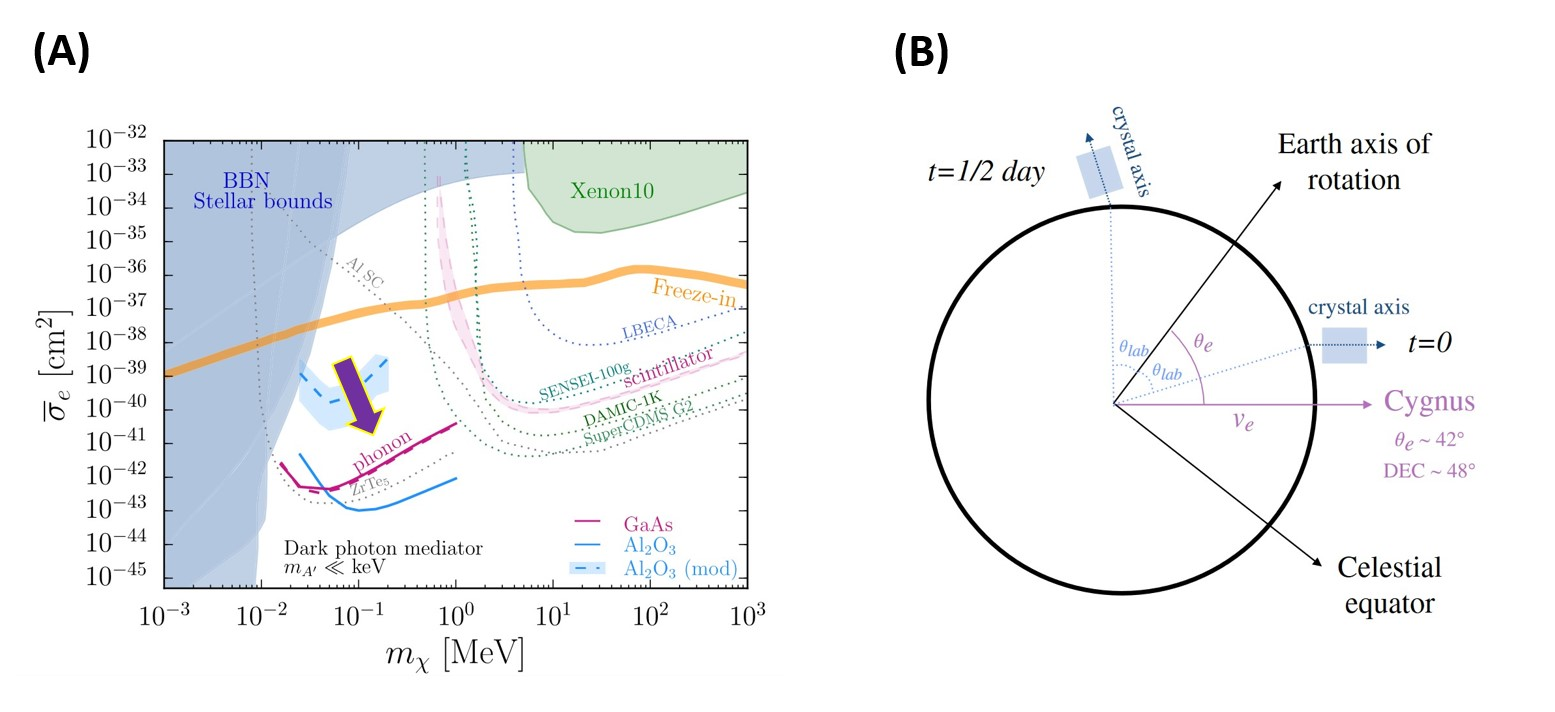
\includegraphics[width=0.9\textwidth]{figures/third_figure.jpg}
    \caption{\textbf{(A)} Cross section of phonon-based dark matter detection, pointed at by purple arrow, along side with other detection techniques (from Ref.\cite{griffin_directional_2018}); \textbf{(B)} An illustration of daily-modulated dark matter signal. The dark matter flux goes through the crystal in different direction at a different time of a day (from Ref.\cite{griffin_directional_2018}).}
    \label{third_figure}
\end{figure}

Recently, a new material, sapphire, has been proposed as suitable material for phonon-based dark matter detection\cite{griffin_directional_2018}. According to this study, sapphire's suitability for phonon-based dark matter detection stems from several factors: (1) As a polar material, sapphire is  expected to interact strongly with dark matter, aided by dark photon mediation; (2) Its insulating nature results in minimal screening effects, potentially enhancing phonon-dark matter interactions; (3) Sapphire's anisotropic property allows for the discrimination of dark matter particles from other types of particles. The anisotropy implies that both electron-phonon coupling and dark-matter-phonon coupling are direction-dependent\cite{griffin_directional_2018}, leading to an anisotropic cross section for dark matter detection. Due to the Earth's rotation, the dark matter signal is expected to vary throughout the day as the direction of dark matter flux changes, depending on the orientation of the Earth. This daily-modulated property enables us to distinguish dark matter signal from other background noise.

The first step towards detecting sub-MeV dark matter is to measure the electron-phonon coupling in sapphire, on the assumption that this coupling mirrors the dark-matter-phonon interaction. \textit{Therefore, we propose conducting a RIXS measurement on sapphire to extract the electron-phonon coupling in different orientation.}  We expect to observe an anisotropic behavior in the phonon signal in RIXS spectrum. Afterwards, we will carefully extract the electron-phonon coupling based on Ament model\cite{ament_determining_2011}. This investigation represents a foundational step in our journey towards dark matter detection.


\section{Planned Research Activities and Schedule}
\paragraph{Project 1: Charge and Lattice Dynamics in Cuprate Superconductors}
We have completed the initial experimental phase of the first project, which involved RIXS measurements on $\mathrm{La_{1.8-x}Eu_{0.2}Sr_xCuO_{4}}$ (with $x=0.125$) Diamond Light Source's I21 beamline in the UK. More experiment might be needed due to the lack of data of $\mathrm{La_{1.8-x}Eu_{0.2}Sr_xCuO_{4}}$ with different doping level. We plan to apply for beamtime at I21 again in the next application cycle. Detailed schedule is as follows
\begin{itemize}
  \item \textit{Pre-grant period}: Collecting RIXS data of $\mathrm{La_{1.675}Eu_{0.2}Sr_{0.125}CuO_{4}}$ at Oxygen-K edge at beamline I21 at Diamond Light Source, focusing primarily on the temperature dependence of charge order and phonon. 
  \item \textit{First phase, Mar.2024 -- Sept.2024}: Analyzing data to extract electron-phonon coupling, simulating charge order and phonon spectrum, and characterizing charge order excitations. In the meantime, we will apply for additional beamtime for further RIXS experiments on $\mathrm{La_{1.8-x}Eu_{0.2}Sr_xCuO_{4}}$ with different doping levels. 
  \item \textit{Second phase, Sept.2024 -- Mar.2025}: Preparing $\mathrm{La_{1.8-x}Eu_{0.2}Sr_xCuO_{4}}$ samples with different doping for subsequent RIXS experiments. 
  \item \textit{Third phase, Mar.2025 -- Sept.2025}: Wrapping up,  finalizing results and drafting the manuscript for publication.
\end{itemize}

\paragraph{Project 2: Electron-Phonon Coupling in KTO and STO}
The proposal of $\mathrm{SrTiO_{3}}$ has been submitted to beamline I21 at Diamond Light Source, and was accepted earlier by the time of this application. The date of the beamtime has not been scheduled yet, but it is most likely to be in 2024. The proposal of $\mathrm{KTaO_{3}}$ has been submitted to beamline 41A at Taiwan Photon Source in Taiwan. 
\begin{itemize}
  \item \textit{Pre-grant period}: Applying for a beamtime at I21 (Diamond Light Source) and 41A (Taiwan Photon Source).
  \item \textit{First phase, Feb.2024 -- Sept.2024}: Preparing Samples and conducting RIXS experiment on $\mathrm{SrTiO_{3}}$ at I21 and $\mathrm{KTaO_{3}}$ at 41A. 
  \item \textit{Second phase, Sept.2024 -- Mar.2025}: Data analysis, extracting electron-phonon coupling in both $\mathrm{SrTiO_{3}}$ and $\mathrm{KTaO_{3}}$. Examining the reverse isotope effect and the anisotropic feature.
  \item \textit{Third phase, Mar.2025 -- post-grant period}:  Wrapping up,  finalizing results and preparing the manuscript for publication.
\end{itemize}

\paragraph{Project 3: Sub-MeV Dark Matter Detection}
The initial experiment on sapphire has been conducted at beamline 41A of Taiwan Photon Source in Taiwan ealier by the time of this application. However, more experiments are needed due to the lack of data in other directions and high-resolution data for (001) orientation. We intend to apply for additional beamtime at beamline ID32 of ESRF in France in the upcoming application cycle.
\begin{itemize}
  \item \textit{Pre-grant period}: Performing initial experiment at beamline 41A, focusing on sapphire orientations $(0001)$, $(1\bar{1}02)$, and $(100)$. 
  \item \textit{First phase, Feb.2024 -- Sept.2024}: Applying for beamtime. Preparing Samples with orientation $(1\bar{1}00)$, $(21\bar{1}0)$, and $(100)$. 
  \item \textit{Second phase, Sept.2024 -- Mar.2025}: Conducting RIXS measurements on the prepared sapphire samples: $(1\bar{1}00)$, $(21\bar{1}0)$, and $(100)$. 
  \item \textit{Third phase, Mar.2025 -- post-grant period}: Data analysis, extracting electron-phonon coupling of all orientations we examined in sapphire.
\end{itemize}

\section{Available Resources}
All three projects require the use of RIXS instruments and high-quality samples. Access to synchrotron facilities and RIXS instruments hinges on successful approval of corresponding research proposals. The proposals are accepted in two cycles annually. Our group, led by Prof. Johan Chang, is known for the high success rate (60-70\%) in securing RIXS proposals, bolsters our confidence in accessing these crucial resources. No major difficulties in getting access to beamtime are foreseen. 

Samples are obtained from different sources: (1) High-quality $\mathrm{La_{1.8-x}Eu_{0.2}Sr_xCuO_{4}}$ (LESCO) samples are provided by Prof. Tohru Kurosawa from Muroran Institute of Technology, with whom we have long-standing collaboration. The samples obtained from him have already been used in Multiple studies\cite{choi2022unveiling,wang_charge_2021} in Prof. Chang's group. We also have the required expertise for precise polishing or cleaving of LESCO samples. (2) $\mathrm{SrTiO_{3}}$ (STO) and $\mathrm{KTaO_{3}}$ (KTO) samples are commercially available. we will collaborate with Benoît Fauqué from Collège de France, a renowned expert in oxide materials. His team will assist in characterizing these samples. (3) Moreover, high-quality single-crystal well-polished sapphire samples, essential for our dark matter detection project, are also commercially available. We have the flexibility to procure these from various manufacturers. 

In our labs, samples can be well characterized, and finely aligned using Laue diffraction. Additionally, we have access to a SQUID magnetometer for magnetic susceptibility measurements and a Physical Property Measurement System (PPMS) for resistivity assessments.

For computational needs, our primary tool is a standard laptop, sufficient for most simulations. For more demanding computational tasks, we have access to the University of Zurich's science cluster\footnote{https://www.zi.uzh.ch/en/teaching-and-research/science-it/computing/sciencecluster.html}, which boasts high-performance GPUs and CPUs.

%Group of Johan chang has great success rate in the accpetance of RIXS proposal (60-70\%).  

%laptop is enough for simulation. in case too heavy, we have access to the cluster. The University of Zürich has a dedicated cluster that features high-performance GPUs and CUPs already used by the hosting group for previous research (https://www.zi.uzh.ch/en/teaching-and-research/science-it/computing/sciencecluster.html) 

%Samples will be obtained from diff sources, will be characterized and prepared in our labs, we will do Laue, they will be aligned with Laue diffraction; a SQUID magnetometer for magnetic susceptibility measurements, and a PPMS for resistivity measurements

%LSCO will be polished/cleaved depending on the needs. We have expertise in our group. sapphire is already polished by the manufactor and KTO/STo as well. 

%LSCO samples from Prof. Tohru Kurosawa cite papger from J Choi PRL 2022, 2008 from Leo's FK application, 

%Sapphire samples: High-quality sapphire single crystal commercially available, we can buy from different manifacture. 

%STO/KTOsamples from Benoit Fauque from https://orcid.org/0000-0002-3855-8371 they are also commercial available, but they will be characterized by B. F. who is an expertise in oxide, we colabourate with them.


Moreover, the machine learning project carried out in the group of Prof. Johan Chang at University of Zurich will greatly facilitate the experiment measurement and the data analysis afterwards. RIXS is now a crucial method for examining quantum materials, but its effectiveness is significantly hampered by the lengthy duration required for data acquisition and the relatively short allocation of beamtime. This machine learning project provides a way to denoise the RIXS data, and thus will be very helpful in accelerating the data acquisition process.  


\section{Significance of Expected Results}

The proposed research projects hold significant implications in the fields of condensed matter physics and dark matter detection. The comprehensive exploration of electron-phonon coupling in different systems through the advanced RIXS technique will certainly provide deeper insights across multiple domains.

\paragraph{Revealing the Nature of Charge Order Excitations in Cuprate Superconductors} While static charge order has been studied extensively in cuprate, dynamical charge order, or charge order excitations, is still not well explored due to the lack of experimental techniques before the advent of RIXS\cite{li_multiorbital_2020}. Thanks to the recent development in RIXS, it is now possible to study the charge order excitations in cuprate superconductors. Our research will provide a new perspective on the relation between phonon and charge order excitations in cuprate superconductors, and thus deepen our understanding of the interplay among phonon, charge order, and superconductivity. 

\paragraph{Advancing Understanding in High-Temperature Superconductivity}
The investigation of electron-phonon coupling in cuprate superconductors, $\mathrm{SrTiO_{3}}$ and $\mathrm{KTaO_{3}}$ is fundamental to unraveling the mysteries of high-temperature superconductivity. Current theories on unconventional superconductivity remain incomplete. Our research aims to bridge this knowledge gap, offering a deeper comprehension of the underlying mechanisms. We anticipate contributions to the understanding of the role played by electron-phonon coupling in unconventional superconductivity, potentially leading to new theoretical frameworks. 

\paragraph{Contributions to Dark Matter Research}
Our investigation into the electron-phonon coupling in sapphire as a candidate for dark matter detection represents a pioneering effort in the search for dark matter. By carefully characterizing electron-phonon interaction, and potentially dark-matter-phonon couplings, this project could significantly impact the design and sensitivity of future phonon-based dark matter detection experiments. This is undoubtedly the first step towards unmasking one of the most important problems in modern physics.

\paragraph{Methodological Advancements}
This research will also demonstrate the capabilities of RIXS as a tool for studying charg order and electron-phonon interactions. We not only aim to make use of the technique experimentally, but also computationally and threotically. We are looking to pushing the boundaries of this technique, developing new simulation method for more accurate extraction of electron-phonon coupling. This will certainly enhance the methodological framework available to the scientific community, potentially leading to new applications of RIXS in other areas of physics and materials science.

\paragraph{Providing data set for machine learning}
Due to the fact that the three projects are all based on RIXS measurements, it creates a playground and provides great opportunity for advancing the denoising technique based on machine learning developed in the group of Prof. Johan Chang at University of Zurich. The denoising technique will be very helpful in accelerating the data acquisition process, and thus will be promising in facilitating future RIXS experiments.



\bibliographystyle{unsrt}
\bibliography{ref}
\addcontentsline{toc}{chapter}{References}

\end{document}
